%**************************************************************************************
% License:
% CC BY-NC-SA 4.0 (http://creativecommons.org/licenses/by-nc-sa/4.0/)
%**************************************************************************************

\documentclass[notes]{beamer}

\mode<presentation> {

\usetheme{Madrid}

% Burnt orange
\definecolor{burntorange}{rgb}{0.8, 0.33, 0.0}
\colorlet{beamer@blendedblue}{burntorange}
% Pale yellow
\definecolor{paleyellow}{rgb}{1.0, 1.0, 0.953}
\setbeamercolor{background canvas}{bg=paleyellow}
% Secondary and tertiary palett
\setbeamercolor*{palette secondary}{use=structure,fg=white,bg=burntorange!80!black}
\setbeamercolor*{palette tertiary}{use=structure,fg=white,bg=burntorange!60!black}

% To remove the footer line in all slides uncomment this line
%\setbeamertemplate{footline}
% To replace the footer line in all slides with a simple slide count uncomment this line
%\setbeamertemplate{footline}[page number]

% To remove the navigation symbols from the bottom of all slides uncomment this line
%\setbeamertemplate{navigation symbols}{}
}

\usepackage{amsmath}
\usepackage{bm}
\usepackage{breqn}
\usepackage{fontawesome}
\usepackage{graphicx} % for figures
\usepackage{subcaption} % for subplots 
\usepackage[labelsep=space,tableposition=top]{caption}
\renewcommand{\figurename}{Fig.} 
\usepackage{cleveref}
\usepackage{caption,subcaption}% http://ctan.org/pkg/{caption,subcaption}
\usepackage{booktabs} % Allows the use of \toprule, \midrule and \bottomrule in tables
\usepackage{multirow}
\usepackage{xcolor}
\usepackage{empheq}
\usepackage[most]{tcolorbox}
\usepackage{listings}% http://ctan.org/pkg/listings
\lstset{basicstyle=\ttfamily,breaklines=true}
\usepackage{siunitx}
\usepackage{verbatim}

% To print 2 slides on a page
%\usepackage{handoutWithNotes}
%\pgfpagesuselayout{2 on 1}[border shrink=2mm]
%----------------------------------------------------------------------------------------
%	TITLE PAGE
%----------------------------------------------------------------------------------------
% The short title appears at the bottom of every slide, the full title is only on the title page
\title[CE 311K: Linear Systems]{CE 311K: Linear System of Equations} 
\author{Krishna Kumar} % name
\institute[UT Austin] % institution 
{
University of Texas at Austin \\
\medskip
\href{mailto:krishnak@utexas.edu}{krishnak@utexas.edu} % email address
}
\date{} % Date, can be changed to a custom date

\begin{document}

\begin{frame}
\titlepage % title page as the first slide
\end{frame}

\newif\ifshowtoc
\showtoctrue% toggles to show the toc

\AtBeginSection{%
	\ifshowtoc
	\begin{frame}
		\tableofcontents[currentsection, subsectionstyle=show/show/hide]
	\end{frame}
	\fi
}

%----------------------------------------------------------------------------------------
% slides
%----------------------------------------------------------------------------------------
%------------------------------------------------

\section{Linear System of Equations}
%------------------------------------------------
\begin{frame}
	\frametitle{Linear System of Equations}
	\begin{figure}[ht]
		\centering
		\includegraphics[width=0.7\textwidth]{figs/linear-systems.png}
	\end{figure}
\end{frame}

%------------------------------------------------
\begin{frame}
	\frametitle{Linear System of Equations: Traffic flow}
	\begin{figure}[ht]
		\centering
		\includegraphics[width=0.7\textwidth]{figs/traffic-flow.png}
	\end{figure}
\end{frame}

%------------------------------------------------
\begin{frame}
	\frametitle{Solving Linear System of Equations}
	\begin{align*}
		3 x_1 + 2 x_2 & = 18 \\
		-x_1 + 2 x_2 & = 2
	\end{align*}
\end{frame}

%------------------------------------------------
\begin{frame}
	\frametitle{Solving Linear System of Equations}
	\begin{figure}[ht]
		\centering
		\includegraphics[width=0.5\textwidth]{figs/graphical-linear-systems.png}
	\end{figure}
\end{frame}

%------------------------------------------------
\begin{frame}
	\frametitle{Singularity and Ill-conditioned}
	\mode<beamer>{
	\begin{figure}[ht]
		\centering
		\includegraphics[width=\textwidth]{figs/singular-illconditioned.png}
	\end{figure}
	}
\end{frame}

\note{A singular matrix is a square matrix which is not invertible. 
	Alternatively, a matrix is singular if and only if it has a determinant of 0.}

%------------------------------------------------
\begin{frame}
	\frametitle{Solving Linear System of Equations}
	\begin{enumerate}
		\item Direct Methods
		\begin{enumerate}
			\item Gauss Elimination
			\item Gauss-Jordan Elimination
			\item LU decomposition
		\end{enumerate}
		\item Iterative Methods
		\begin{enumerate}
			\item Jacobi iterative
			\item Gauss-Seidel
		\end{enumerate}
	\end{enumerate}
\end{frame}

%------------------------------------------------
\begin{frame}
	\frametitle{Direct methods}
	Consider a system of 3 linear equations for simplicity:
	\begin{align*}
	a_{11} x_1 + a_{12} x_2 + a_{13} x_3 & = b_1 \\
	a_{21} x_1 + a_{22} x_2 + a_{23} x_3 & = b_2 \\
	a_{31} x_1 + a_{32} x_2 + a_{33} x_3 & = b_3
	\end{align*}
	Matrix form is:
	\begin{align*}
		\begin{bmatrix}
		a_{11} & a_{12} & a_{13} \\
		a_{21} & a_{22} & a_{23} \\
		a_{31} & a_{32} & a_{33} \\
		\end{bmatrix}
		\begin{bmatrix}
		x_1 \\
		x_2 \\
		x_3 \\
		\end{bmatrix} = 
		\begin{bmatrix}
		b_1 \\
		b_2 \\
		b_3 \\
		\end{bmatrix}
	\end{align*}
	Concise form: $A x = b$
	
\end{frame}

%------------------------------------------------
\begin{frame}
	\frametitle{Systems that can be solved easily}

	\begin{align*}
	\begin{bmatrix}
	a_{11} & a_{12} & a_{13} \\
	0 & a_{22} & a_{23} \\
	0 & 0 & a_{33} \\
	\end{bmatrix}
	\quad
	\begin{bmatrix}
	a_{11} & 0 & 0 \\
	a_{21} & a_{22} & 0 \\
	a_{31} & a_{32} & a_{33} \\
	\end{bmatrix}
	\quad
	\begin{bmatrix}
	a_{11} & 0 & 0 \\
	0 & a_{22} & 0 \\
	0 & 0 & a_{33} \\
	\end{bmatrix}
	\end{align*}
\end{frame}


%------------------------------------------------
\begin{frame}
	\frametitle{Solve by ``back substitution' Upper triangle system (U)}
	
	\begin{align*}
	\begin{bmatrix}
	a_{11} & a_{12} & a_{13} \\
	0 & a_{22} & a_{23} \\
	0 & 0 & a_{33} \\
	\end{bmatrix}
	\begin{bmatrix}
	x_1 \\
	x_2 \\
	x_3 \\
	\end{bmatrix}
	\begin{bmatrix}
	b_1 \\
	b_2 \\
	b_3 \\
	\end{bmatrix}
	\end{align*}
	\mode<beamer>{
	Start with the last equation 3:
	$x_3 = b_3 / a_{33}$
	
	Equation 2: $a_{22}x_2 + a_{23}x_3 = b_2$ so
	\begin{equation*}
	x_2 = \frac{b_2 - a_{23}x_3}{a_{22}}
	\end{equation*}
	
	Equation 1: $a_{11}x_1 + a_{12}x_2 + a_{13} x_3 = b_1$ so
	\begin{equation*}
	x_1 = \frac{b_1 - (a_{12}x_2 + a_{13}x_3)}{a_{11}}
	\end{equation*}
	General for `n` systems: $x_n = b_n/a_{nn}$
	$x_i = \frac{b_i - \sum_{j = i+1}^{n}{a_{ij} x_j}}{a_{ii}}$
	}
\mode<handout>{\vspace{5cm}}
\end{frame}


%------------------------------------------------
\begin{frame}
	\frametitle{Gauss Elimination}
	Consider a system of 3 linear equations:
	\begin{align*}
	\begin{bmatrix}
		2 & 4 & 6 \\
		4 & 11 & 21 \\
		6 & 21 & 52 \\
	\end{bmatrix}
	\begin{bmatrix}
		x_1\\
		x_2\\
		x_3\\
	\end{bmatrix}
	\begin{bmatrix}
		24 \\
		72 \\
		158 \\
	\end{bmatrix}
	\end{align*}
	\mode<beamer>{
	Divide row 2 by -2 and row 3 by -3
	\begin{align*}
		\begin{bmatrix}
			2 & 4 & 6 \\
			0 & 3 & 9 \\
			0 & 9 & 34 \\
		\end{bmatrix}
		\begin{bmatrix}
			x_1\\
			x_2\\
			x_3\\
		\end{bmatrix}
		\begin{bmatrix}
			24 \\
			24 \\
			86 \\
		\end{bmatrix}
	\end{align*}
	Second reduction:
	\begin{align*}
	\begin{bmatrix}
	2 & 4 & 6 \\
	0 & 3 & 9 \\
	0 & 0 & 7 \\
	\end{bmatrix}
	\begin{bmatrix}
	x_1\\
	x_2\\
	x_3\\
	\end{bmatrix}
	\begin{bmatrix}
	24 \\
	24 \\
	14 \\
	\end{bmatrix}
	\end{align*}
	$x_3 = 2, x_2 = 2, x_1 = 2$
	}
	\mode<handout>{
		\vspace{5cm}
	}
\end{frame}
\note{
	a = np.array([[2,4,6], [4,11,21], [6, 21, 52]])
	
	b = np.array([24, 72, 158])
	
	x = np.linalg.solve(a, b)
}



%------------------------------------------------
\begin{frame}
	\frametitle{Gauss Elimination: Limitations}
	\begin{enumerate}
		\item Prone to round off errors, when we have many ($>100$) equations.
		\item If coefficient matrix is sparse (lots of zeros), elimination methods are very inefficient.
	\end{enumerate}
\end{frame}


%------------------------------------------------
\begin{frame}
	\frametitle{Gauss Seidel Iterative approach}
	 For conciseness, we limit to $3\times3$ equations. If diagonal elements are all non-zero, then the equations can be solved as:
		\begin{align*}
	\begin{bmatrix}
	a_{11} & a_{12} & a_{13} \\
	a_{21} & a_{22} & a_{23} \\
	a_{31} & a_{32} & a_{33} \\
	\end{bmatrix}
	\begin{bmatrix}
	x_1 \\
	x_2 \\
	x_3 \\
	\end{bmatrix} = 
	\begin{bmatrix}
	b_1 \\
	b_2 \\
	b_3 \\
	\end{bmatrix}
	\end{align*}
	\mode<beamer>{
		\begin{align*}
		x_1 & = \frac{b_1 - a_{12}x_2 - a_{13}x_3}{a_{11}} \\
		x_2 & = \frac{b_2- a_{21}x_1 - a_{23}x_3}{a_{22}} \\
		x_3 & = \frac{b_3 - a_{31}x_1 - a_{32}x_2}{a_{33}} \\
		\end{align*}
	}
	\mode<handout>{
		\vspace*{3cm}
	}
\end{frame}

%------------------------------------------------
\begin{frame}
	\frametitle{Gauss Seidel Iterative approach}
	Using Gauss-Seidel solve for [x]
	\begin{align*}
	4x_1 + x_2   + 2x_3 & = 4
\\
	3x_1 + 5 x_2 + x_3 & = 7
\\
	x_1  + x_2   + 3x_3 & = 3 \\
	\end{align*}
	\mode<beamer>{
		Assuming an initial guess of $x_1, x_2, x_3 = 0$. End of first iteration.
\begin{align*}
x_1 & = \frac{4 - x_2 - 2x_3}{4} = \frac{4 - 0 - 0}{4} = 1 \\
x_2 & = \frac{7 - 3x_1 - x_3}{5} = \frac{7 - 3 * 1 - 0}{5} = 0.8 \\
x_3 & = \frac{3 - x_1 - x_2}{3} = \frac{3 - 1 - 0.8}{3} = 0.4 \\
\end{align*}
	}
	\mode<handout>{
		\vspace*{3cm}
	}
\end{frame}

%------------------------------------------------
\begin{frame}
	\frametitle{Gauss Seidel Iterative approach}
	Using Gauss-Seidel solve for [x]
	\mode<beamer>{
		End of first iteration:  $x_1, x_2, x_3 = 1, 0.8, 0.4$
		\begin{align*}
			x_1 & = \frac{4 - x_2 - 2x_3}{4} = \frac{4 - 0.8 - 2*0.4}{4} = 0.6 \\
			x_2 & = \frac{7 - 3x_1 - x_3}{5} = \frac{7 - 3 * 0.6 - 0.4}{5} = 0.96 \\
			x_3 & = \frac{3 - x_1 - x_2}{3} = \frac{3 - 0.6 - 0.96}{3} = 0.48 \\
		\end{align*}
		End of first iteration:  $x_1, x_2, x_3 = 0.6, 0.96, 0.48$
		\begin{align*}
			x_1 & = \frac{4 - x_2 - 2x_3}{4} = \frac{4 - 0.96 - 2*0.48}{4} = 0.52 \\
			x_2 & = \frac{7 - 3x_1 - x_3}{5} = \frac{7 - 3 * 0.52 - 0.48}{5} = 0.992 \\
			x_3 & = \frac{3 - x_1 - x_2}{3} = \frac{3 - 0.52 - 0.992}{3} = 0.496 \\
		\end{align*}
	}
	\mode<handout>{
	End of first iteration:  $x_1, x_2, x_3 = 1, 0.8, 0.4$
	\begin{align*}
		x_1 & = \frac{4 - x_2 - 2x_3}{4} =  \\
		x_2 & = \frac{7 - 3x_1 - x_3}{5} = \\
		x_3 & = \frac{3 - x_1 - x_2}{3} = \\
	\end{align*}
	End of first iteration:  $x_1, x_2, x_3 = 0.6, 0.96, 0.48$
	\begin{align*}
		x_1 & = \frac{4 - x_2 - 2x_3}{4} = \\
		x_2 & = \frac{7 - 3x_1 - x_3}{5} = \\
		x_3 & = \frac{3 - x_1 - x_2}{3} =  \\
	\end{align*}
	}
\end{frame}


%------------------------------------------------
\begin{frame}
	\frametitle{Gauss Seidel Convergence criteria}
	Convergence can be checked using the relative error.
	\begin{align*}
	\left|\varepsilon_{a, i}\right| = \left|\frac{x_i^k - x_i^{k-1}}{x_i^k}*100\% \right|< \varepsilon_s
	\end{align*}
	where $k$, and $k-1$ represents the current and previous iterations
\end{frame}

\note{
	Gauss-Seidel only works for diagonally dominant matrix
}



%------------------------------------------------
\begin{frame}
	\frametitle{Gauss Seidel: Disney force diagram}
		\begin{figure}[ht]
			\centering
			\includegraphics[width=\textwidth]{figs/freebody.png}
		\end{figure}
\end{frame}


%------------------------------------------------
\begin{frame}
	\frametitle{Gauss Seidel: Disney force diagram}
		\begin{figure}[ht]
			\centering
			\includegraphics[width=\textwidth]{figs/freebody-empty.png}
		\end{figure}		
\end{frame}



%------------------------------------------------
\begin{frame}
	\frametitle{Gauss Seidel: Disney force diagram}
	\begin{table}[]
		\begin{tabular}{lcc}
			\toprule
			\textbf{Character} & \textbf{Mass (kg)} & \textbf{Drag coefficient (kg/s)} \\
			\midrule
			Sven               & 100                & 40                               \\
			Anna               & 60                 & 25                                \\
			Olaf               & 15                 & 10                               \\
			\bottomrule
		\end{tabular}
	\end{table}
\end{frame}

%------------------------------------------------
\begin{frame}
	\frametitle{Gauss Seidel: Disney force diagram}
	Free-body diagram, moving with a constant velocity $v = 5 m/s$. compute the acceleration and forces. Unknowns are $a, T, R$.
	\begin{align*}
		m_1 g - T - c_1 * v & = m_1 a \\
		m_2 g + T - c_2 * v - R &= m_2 a \\
		m_3 g     - c_3 * v + R & = m_3 a \\
	\end{align*}
	\begin{align*}
	m_1 a + T & = m_1 g - c_1 * v \\
	m_2 a - T + R &= m_2 a - c_2 * v \\
	m_3 a     - R & = m_3 a - c_3 * v \\
	\end{align*}
	\begin{align*}
		100 a + T & = 1000 - 40 * 5 = 800\\
		60 a - T + R &= 600 - 25 * 5  = 475\\
		15 a     - R & = 150 - 10 * 5 = 100 \\
	\end{align*}
\end{frame}

%------------------------------------------------
\begin{frame}
	\frametitle{Gauss Seidel: Disney force diagram}
	Free-body diagram, moving with a constant velocity $v = 5 m/s$. compute the acceleration and forces. Unknowns are $a, T, R$.
	\begin{align*}
		\begin{bmatrix}
			100 & 1 & 0 \\
			60 & -1 & 1 \\
			15 & 0 & -1 \\
		\end{bmatrix}
		\begin{bmatrix}
			a \\
			T \\
			R \\
		\end{bmatrix} = 
		\begin{bmatrix}
		800 \\
		475 \\
		100 \\
	\end{bmatrix}
	\end{align*}

	The acceleration $a = 7.8571428 m/s^2$, $T= 14.29N$, and $R=17.86 N$.
\end{frame}
%------------------------------------------------
\begin{frame}
	\frametitle{3-noded Truss analysis}
	\begin{figure}[ht]
		\centering
		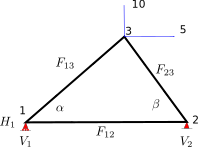
\includegraphics[width=0.5\textwidth]{figs/3truss.png}
	\end{figure}
	\vspace{4cm}
\end{frame}

%------------------------------------------------
\begin{frame}
	\frametitle{3-noded Truss analysis}
	\begin{figure}[ht]
		\centering
		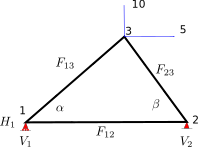
\includegraphics[width=0.5\textwidth]{figs/3truss.png}
	\end{figure}
	\vspace{4cm}
\end{frame}


%------------------------------------------------
\begin{frame}
	\frametitle{3-noded Truss analysis}
	\begin{figure}[ht]
		\centering
		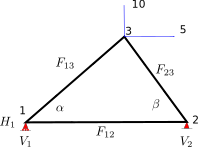
\includegraphics[width=0.5\textwidth]{figs/3truss.png}
	\end{figure}
	\vspace{4cm}
\end{frame}


%------------------------------------------------
\begin{frame}
	\frametitle{3-noded Truss analysis}
	\vspace{4cm}
\end{frame}

%------------------------------------------------
\begin{frame}
	\frametitle{3-noded Truss analysis}
	\vspace{4cm}
\end{frame}



\note{
	\begin{figure}[ht]
		\centering
		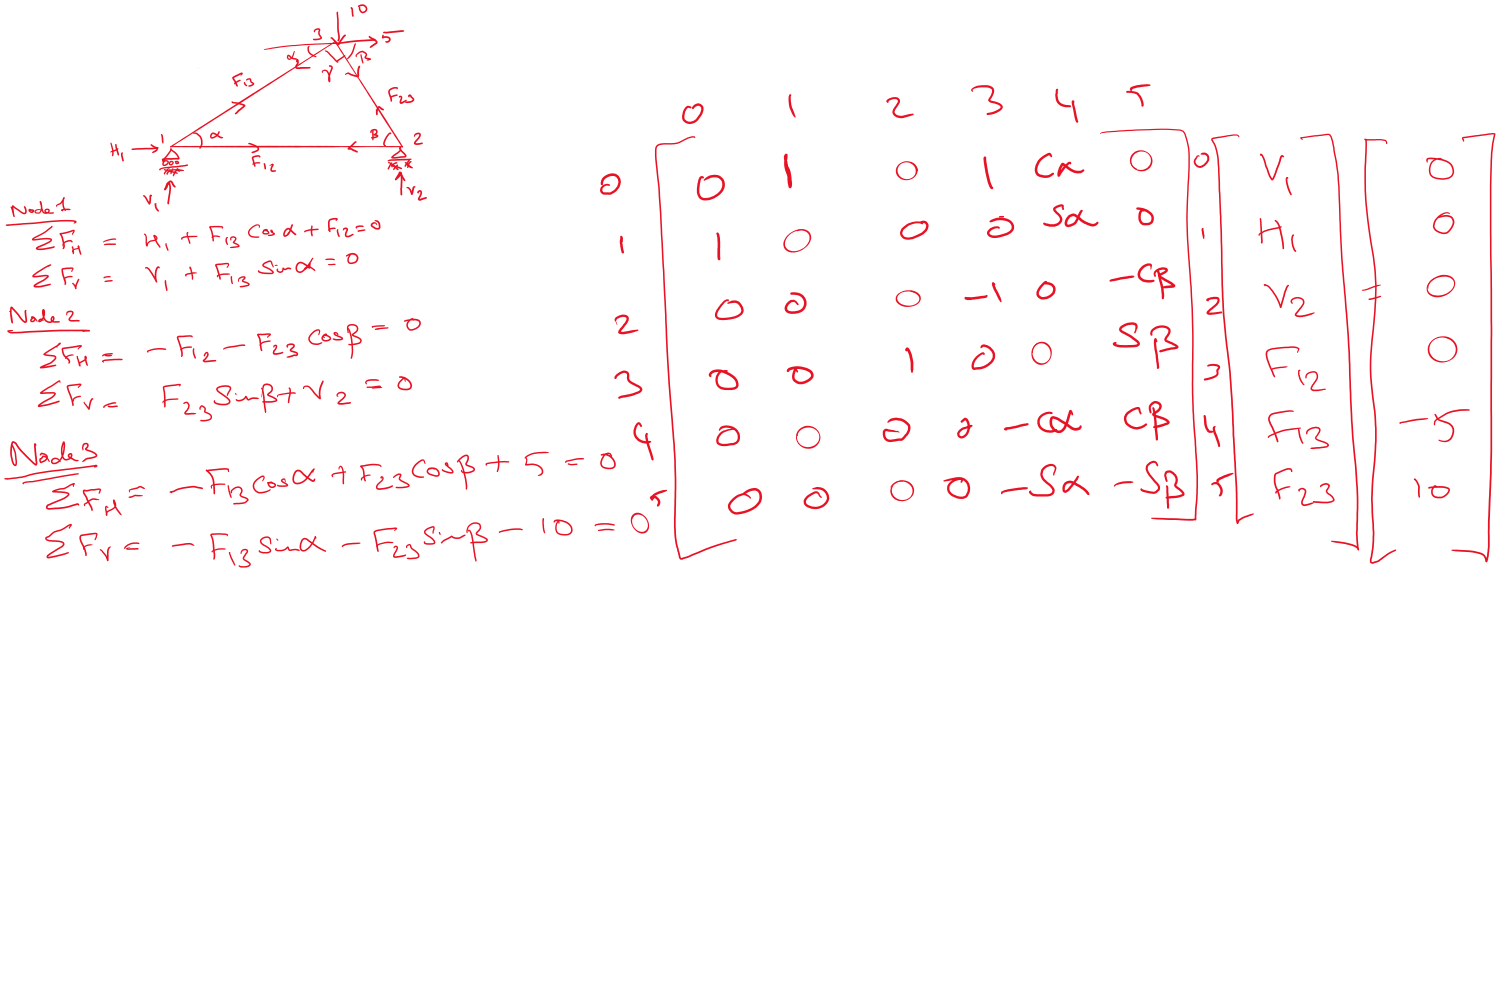
\includegraphics[width=\textwidth]{figs/3node-truss-analysis.png}
	\end{figure}
}e
%------------------------------------------------
\begin{frame}
	\frametitle{Truss analysis}
	\begin{figure}[ht]
		\centering
		\includegraphics[width=\textwidth]{figs/truss.png}
	\end{figure}
\end{frame}

%------------------------------------------------
\begin{frame}
	\frametitle{Truss analysis: Force balance}
	\begin{figure}[ht]
		\centering
		\includegraphics[width=0.8\textwidth]{figs/force-balance.png}
	\end{figure}
\end{frame}

%------------------------------------------------
\begin{frame}
	\frametitle{Truss analysis: Matrix formulation}
	\begin{figure}[ht]
		\centering
		\includegraphics[width=\textwidth]{figs/truss-matrix.png}
	\end{figure}
\end{frame}

\end{document}
